\chapter{Energy-Based Models (EBM)}

I modelli basati sull'energia (Energy-Based Models, EBM) costituiscono un paradigma di modellazione che si distacca dai classici approcci discriminativi o generativi che conosciamo grazie al corso di Machine Learning. Invece di apprendere direttamente una funzione esplicita di predizione normalizzata, un \textbf{EBM} definisce un'\textit{energia} associata a ogni configurazione possibile di input $x$ e output $y$, misurandone la compatibilità. Questa energia viene definita tramite una funzione scalare $E(x, y)$, il quale obbiettivo diventa minimizzarla, e viene definito come \textit{obbiettivo inferenziale}. Gli \textbf{Energy Based Model}, si articolano principalmente in due fasi, quella di allenamento, solitamente molto costosa e quella di inferenza. 

\section{Training}
Nella prima fase, il modello impara la funzione d'energia tramite l'uso di un input e di un'etichetta di riferimento, l’idea chiave è di definire un’energia associata a ogni configurazione possibile degli input (e, se presenti, degli output), dove le configurazioni "plausibili" hanno energia bassa mentre le configurazioni "implausibili" hanno energia alta. Allenare un EBM richiede di minimizzare un loss che coinvolge questa energia, spesso confrontando l’energia di esempi reali con quella di esempi generati.
\section{Inferenza}
Una volta che il modello è stato allenato, possiamo usarlo per fare inferenza, ossia determinare quale output y (o quale input x) minimizza l’energia, in altre parole, trovare la configurazione più probabile secondo il modello. Ad esempio, in un EBM discriminativo $E(x,y)$, possiamo usare il modello per inferire l’etichetta $y$ più probabile per un dato $x$:

\begin{equation}
    \hat{y} = \arg\min_y E(x, y)
\end{equation}
In molti casi pratici il modello EBM è già allenato da qualcun altro, o con tecniche costose, noi lo usiamo solo per inferneza, cioè non modifichiamo i pesi, ma utiliziamo il modello per selezionare le configurazioni a bassa energia, ad esempio:
\begin{itemize}
    \item Trovare la label più probabile per un'immagine;
    \item Campionare un'immagine simile a un target;
    \item Scegliere tra alternative quella più compatibile con un certo contesto.
\end{itemize}

Il fenomeno dell'inferenza viene solitamente visualizzato tramite un'interpretazione grafica visibile in Figura~\ref{fig:InfGoodBad}, se la superficie è piatta, questo vuol dire che l'allenamento non è stato fatto in maniera corretta poiché non identificherà delle differenze nelle varie zone, differentemente se la superficie risulta essere ricurva, sicuraemente è stato allenato bene, distinguendo varie zone in base alla loro energia, e il passo successivo sarà semplicemente quello di trovare i valori precisi che ci generano il minimo, come spiegato nel passo inferenziale.
\begin{figure}
    \centering
    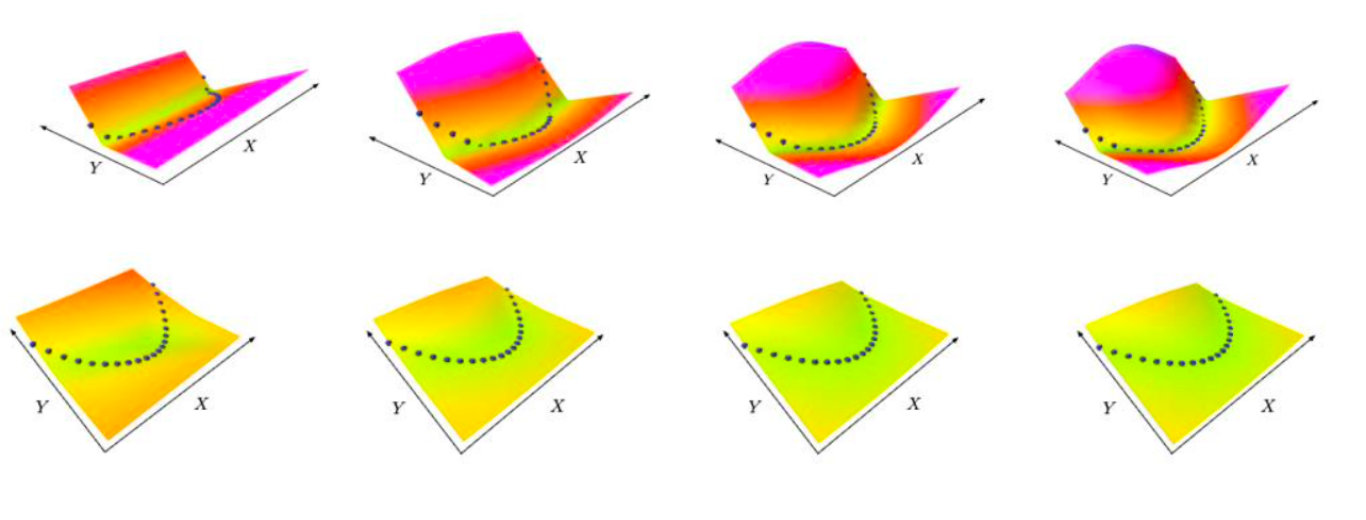
\includegraphics[width=0.7\textwidth]{figure/InferenceGoodBad.png}
    \caption{Sopra possiamo vedere un'esito dell'applicazione dell'inferenza a seguito di un buon training, sotto invece possiamo vedere l'esito a seguito di un pessimo training, poiché ignora gli input e produce valori di output identici, questo risultato la superficie energetica infatti risulta essere sempre piatta e uguale a zero in tutti i punti.}
    \label{fig:InfGoodBad}
\end{figure}

\subsection{Quando usare un EBM}
I casi d'uso degli EBM includono:
\begin{itemize}
    \item Problemi che richiedono calcoli complessi per determinare l'output;
    \item Situazioni con uscite multiple plausibili (es. futuri alternativi);
    \item Inferenza come soddisfacimento di vincoli, tipico di traduzioni linguisticamente corrette o trascrizioni fonetiche coerenti.
\end{itemize}

\section{Modelli espliciti vs impliciti}

Un modello feed-forward classico è una funzione esplicita $y = f(x)$, dunque calcola $y$ a partire da $x$, mentre un EBM definisce una relazione \textit{implicita} tra $x$ e $y$ tramite la funzione $E(x, y)$. L'inferenza consiste nel risolvere l'ottimizzazione rispetto a $y$. Questo consente l'esistenza di molteplici $y$ compatibili con uno stesso $x$, rendendo l'approccio adatto per compiti multimodali. Se $y$ è continuo, è essenziale che $E$ sia differenziabile e liscia, per consentire l'uso di algoritmi di ottimizzazione basati sul gradiente.

\begin{figure}
    \centering
    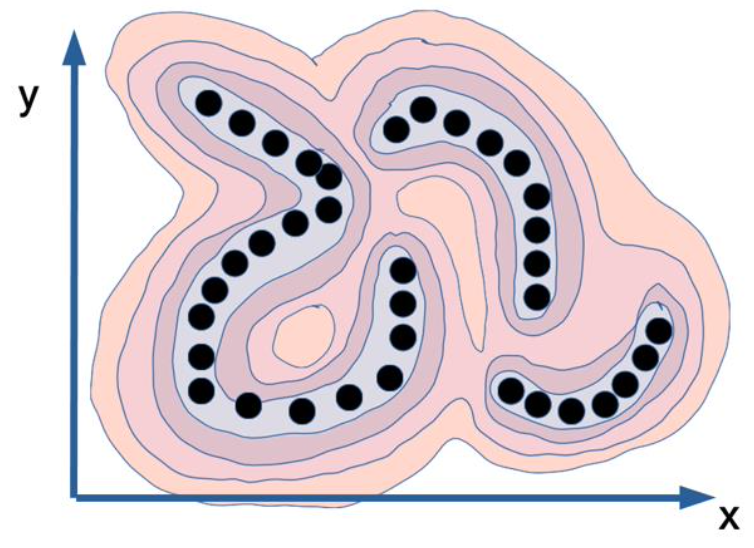
\includegraphics[width=0.7\textwidth]{figure/LowEnHighEn.png}
    \caption{Visualizzazione dell'energia, vicino ai datapoint abbiamo un'energia più bassa, mentre man mano che ci si allontana l'energia aumenta.}
    \label{fig:lEnhEn}
\end{figure}

\section{EBM per predizione multimodale}

Due degli approcci ampiamente utilizzati, ma anche molto diversi fra loro i quali estendono il paradigma classico degli EBMs, sfruttati in particolare in ambiti come multimodalità e modellazione generativa profonda, sono i seguenti:

\begin{itemize}
    \item \textbf{Joint Embedding Architectures}: basate sulla distanza nello spazio delle feature;
    \item \textbf{Latent Variable Models}: introducono variabili latenti per rappresentare fattori di variazione non osservati.
\end{itemize}

\subsection{Joint Embedding}

In un \textbf{Joint Embedding} EBM, si definisce una funzione di energia sullo spazio latente condiviso tra input e output, tipicamente tramite embedding (proiezioni). È utilizzato in modelli contrastivi e multimodali (es. immagine-testo). Algoritmi noti includono Siamese Networks e tecniche di metric learning (\cite{bromley1993signature, chopra2005learning, hadsell2006dimensionality}). Il vantaggio principale è l'assenza di necessità di ricostruzione a livello di pixel. Considerando $x$ come un'immagine di input e $y$ come output testuale e $f(x)$ e $g(y)$ due reti neurali che proiettano $x$ e $y$ in uno spazio comune nella seguente maniera:

\begin{equation}
    E(x,y) = - \langle f(x)\,,\,g(y)\rangle
\end{equation}

L'energia pertanto viene ottenuta come il prodotto scalare o cosine similarity delle due reti neurali, l'energia risulterà di un basso valore se $x$ e $y$ risultassero compatibili fra loro, fornendo una grande similarità. Esempi reali di applicazione includono:
\begin{itemize}
    \item DeepFace~\cite{taigman2014deepface}
    \item PIRL~\cite{misra2019pirl}, MoCo~\cite{he2019moco}
    \item SimCLR~\cite{chen2020simclr}
\end{itemize}

L'obbiettivo finale è ovviamente quello di minimizzare l'energia e dunque massimizzare la similarità per le coppie vere, mentre massimizzare l'energia e minimizzare la similarità per le coppie false.

\subsection{Latent Variable EBMs}
In questa tipoliga di modello vengono sfruttate le variabili latenti $z$, le quali parametrizzano lo spazio delle predizioni. Idealmente rappresentano dei fattori indipendenti, tuttavia la loro capacità informativa deve essere minimizzata in modo tale da evitare che tutta l'informazione della predizione passi da $z$, ma venga solo influenzata parzialmente da essa.

\begin{figure}
    \centering
    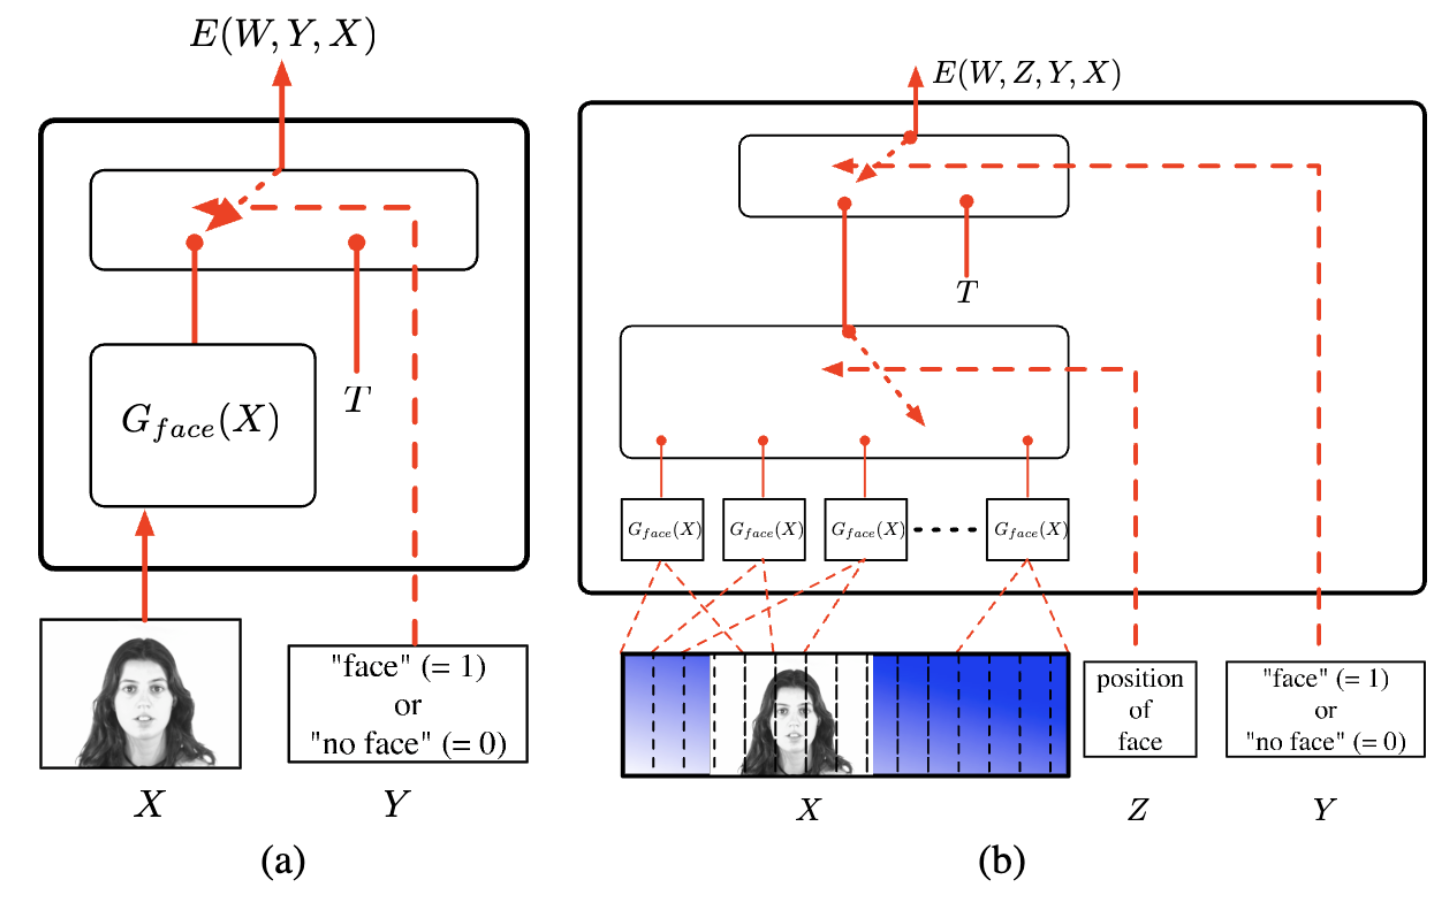
\includegraphics[width=0.6\textwidth]{figure/ebm-face.png}
    \caption{Confronto tra due architetture Energy-Based: (a) un EBM discriminativo semplice, e (b) un EBM con variabile latente. 
    Nel primo caso, la funzione di energia $E(W, Y, X)$ valuta direttamente la compatibilità tra l'immagine $X$ e l'etichetta binaria $Y$. Nel secondo caso, viene introdotta una variabile latente $Z$ che rappresenta la posizione del volto, e il modello calcola l'energia congiunta $E(W, Z, Y, X)$. Questo consente al modello di apprendere rappresentazioni strutturate e di migliorare la localizzazione e classificazione del volto all'interno dell'immagine.}
    \label{fig:ebm-face}
\end{figure}

Alcuni esempi applicativi di questa tipologia di modello si riversano nella lettura di parole scritte a mano, permettendo di sapere dove iniziano e finiscono i caratteri di una parola, ma anche nella comprensione del parlato, riuscendo a segmentare in fonemi o parole un intero discorso, rendendo il tutto molto utile.

\subsection{EBM con variabili latenti condizionali}
Come abbiamo detto precedentemnte nel modello con variabili latenti, vi è il rischio che la variabile latente prenda il soppravvento sulle informazioni fornite in input, pertanto è utile introdurre un regolarizzatore $R(z)$ che limiti la capacità informativa di $z$. Altrimenti, ogni $y$ potrebbe essere ricostruito perfettamente, risultando in una superficie energetica piatta. Alcuni approcci includono:
\begin{itemize}
    \item Quantizzazione/discretizzazione;
    \item Penalizzazioni tipo L0, L1;
    \item Inibizione laterale;
    \item Aggiunta di rumore controllato (es. VAE).
\end{itemize}

\section{Training degli Energy-Based Models}

Per allenare un EBM, si parametrizza la funzione $F(x, y; \theta)$ e si apprendono i parametri $\theta$ usando coppie $(x^{(i)}, y^{(i)})$ osservate. Si desidera:
\begin{equation}
    F(x^{(i)}, y^{(i)}) < F(x^{(i)}, y), \quad \forall y \neq y^{(i)}
\end{equation}

\subsection{Due approcci principali}
\begin{enumerate}
    \item \textbf{Metodi contrastivi:} minimizzano l'energia sulle coppie corrette e la massimizzano su quelle scorrette;
    \item \textbf{Metodi con regolarizzazione o architetturali:} limitano il volume delle regioni a bassa energia.
\end{enumerate}

\subsection{Problemi con il massimo di verosimiglianza}
L'approccio probabilistico cerca di creare un "canyon" infinitamente stretto e profondo attorno alla distribuzione dei dati. Questo rompe la liscezza della funzione energetica, rendendo difficile l'inferenza tramite gradiente. Per ovviare a questo problema, si impiegano approcci regolarizzati.

\subsection{Distribuzione di Gibbs}
In un'ottica probabilistica, l'energia può essere interpretata come negativo del logaritmo di una distribuzione non normalizzata:
\begin{equation*}
    P(y|x) \propto e^{-\beta F(x, y)}.
\end{equation*}

Il parametro $\beta$ è associato alla temperatura (\emph{inverse temperature}). Tuttavia, calcolare la normalizzazione è spesso complesso, perciò è sconsigliato stimare probabilità esplicite almeno che non sia strettamente necessario, poiché la formula è quella visibile di seguito.

\begin{equation}
    P(y\,|\,x)= -\frac{e^{-p\,E(x,y)}}{\int_{y'}e^{-p\,E(x,y')}}
\end{equation}

\section{Contrastive Methods}

Questi metodi allenano $E$ abbassando l'energia delle coppie corrette $(y, W)$ e alzandola per tutte le altre $(Y,W)$. 

\begin{equation}
    P(Y\,|\,W)= -\frac{e^{-\beta\,E(Y,W)}}{\int_{y'}e^{-\beta\,E(y,W)}}
\end{equation}
\begin{equation}
    L(Y,W) = E(Y,W) + \frac{1}{\beta}\,\log\int_ye^{-\beta\,E(y,W)}
\end{equation}

\subsection{Esempi di contrastive training}
\begin{itemize}
    \item Contrastive Divergence con campioni reali e negativi ottenuti via MCMC;
    \item Funzioni di loss con margine non nullo (es. Square-Square, negative log-likelihood);
    \item Embedding contrastivo: distanza tra campioni nello spazio delle feature.
\end{itemize}

\section{Embedding non contrastivo}

Superano il problema del mining dei negativi difficili usando pesi lievemente differenti tra i due rami di una rete siamese. Esempi:
\begin{itemize}
    \item SimSiam~\cite{chen2021simsiam};
    \item BYOL (Bootstrap Your Own Latent).
\end{itemize}

Non trattiamo questi esempi, poiché porterebbero a un livello di dettaglio ulteriore, il quale porterebbe ad andare al di fuori delle competenze richieste dal corso, tuttavia possono essere approfonditi attraverso la lettura dei paper citati.

\section{Self-Supervised Learning (SSL)}

Gli esseri umani apprendono osservando, accumulando conoscenza implicita del mondo. Questo processo è alla base del concetto di self-supervised learning, il quale si basa proprio dalla tipologia di apprendimento seguita dai bambini: osservazioni e piccole interazioni con ciò che li circonda. Questo infatti permette ai bambini di apprendere un enorme quantitativo di informazioni riguardo la struttura del mondo e la fisica intrinseca delle cose. Il \textbf{Self-Supervised Learning} è in grado di predirre qualsiasi parte dell'input a partire da una singola porzione dello stesso, predirre il futuro a partire dal passato, predirre la parte invisibile da quella visibile, essere in grado di predirre le parti mascherate/corrotte a partire da quelle disponibili. Quindi come se fosse in grado di ricostruire qualcosa che manca, avendone già una buona parte, una vera e propria funzione di completamento.

\subsection{Applicazioni di SSL}
Wav2Vec 2.0 si basa proprio su questa tipologia, venendo allenato su 960 ore di testo parlato, non etichettato e allenato in 10 minuti riesce ad eguagliare un modello meno evoluto con lo stesso training set il quale per ottenere le stesse performance dovrebbe essere allenato per ben 100 ore. Modelli come BERT, GPT e simili sono esempi di successo di SSL. Le loro performance su benchmark come RACE dimostrano la potenza della predizione contestuale da input parziali, ottenendo una percentuale di successo che si aggira fra il 45\% e il 90\%.

